%!TEX program = xelatex
\documentclass[12pt,hyperref,a4paper,UTF8]{ctexart}
\usepackage{UIBEReport}

\definecolor{winered}{rgb}{0.5,0,0}
\hypersetup{
  colorlinks = true,
  linkcolor  = {winered},
  citecolor  = {winered},
  urlcolor   = {winered},
}

\title{\songti\bfseries\zihao{2} 国家新一代人工智能创新发展试验区政策对企业研发投入的影响：\\来自多期双重差分的证据\thanks{修订稿一。本稿核对回归输出与图示后，修正了批次样本量、2020年批次占比、安慰剂次数和若干与图不一致的表述，并把总体平均效应的结论收回到“不能拒绝零”。作者简介：陈沫樵，对外经济贸易大学中国金融学院鸿儒2401班本科生，学号202442087。}}
\author{\songti\zihao{4} 陈沫樵}
\date{}

\newtoks\entitle
\newtoks\enauthor
\newtoks\eninstitute
\newtoks\enabstract
\newtoks\enkeywords

\entitle{National AI Innovation Zones and Corporate R\&D Investment:\\
Evidence from Staggered Difference-in-Differences}
\enauthor{Mochiao Chen}
\eninstitute{University of International Business and Economics}
\enabstract{%
Using 4,875 A-share listed firms over 2013--2025, this paper estimates the effect of China's National AI Innovation Zone designations on R\&D intensity. The two-way fixed effects coefficient is 0.0004 ($t=1.38$) and is indistinguishable from zero; capital-expenditure intensity is also unaffected. Event-study confidence intervals cover zero after designation, and the pre-period point estimates are not a flat line at zero. Cohort-specific comparisons against never-treated firms yield positive effects for the 2019 cohort (0.23 percentage points, $t=2.38$) and the 2021 cohort (0.13 percentage points, $t=2.46$), and estimates near zero for 2020 and 2022. The 2020 cohort is 48 percent of treated firms, not 51 percent. The policy response is concentrated in high-AI-exposure industries (interaction $0.0028$, $t=3.74$). A composite subsidy measure moves down, not up. A larger response among high-leverage firms is consistent with a financing channel but does not measure credit costs. In a permutation of treatment timing, the average coefficient exceeds only about 55 percent of placebo draws. The evidence supports heterogeneous and only partly identified responses, not a robust average increase in R\&D.%
}
\enkeywords{AI industrial policy; place-based policy; R\&D; staggered difference-in-differences; China}

\newcommand{\enmaketitle}{%
\vspace{2em}
\begin{center}
{\bfseries \Large \the\entitle}\\
\the\enauthor\\
\small(\the\eninstitute)
\end{center}
\vspace*{-2ex}
\noindent\small\textbf{Summary:}\the\enabstract \\
\textbf{Keywords:} \the\enkeywords
}

\begin{document}
\maketitle

\begin{abstract}
本文使用2013—2025年4,875家A股上市公司、44,594条公司—年度观测，估计国家新一代人工智能创新发展试验区对企业研发强度的影响。研发强度定义为研发支出除以总资产。双向固定效应系数为0.0004（$t=1.38$），不能拒绝平均效应为零；资本支出强度的系数为$-0.0007$（$t=-0.78$）。事件研究里，政策后各期的95\%置信区间都覆盖零，政策前的点估计也不是贴在零上的水平线。

把每个批次只与从未获批城市的企业比较，2019年批次的处理效应为0.0023（399家，$t=2.38$），2021年批次为0.0013（597家，$t=2.46$），2020年与2022年批次接近零。2020年批次有1,167家企业，占处理组2,424家的48.1\%。高人工智能暴露行业与政策的交互项为0.0028（$t=3.74$）。补贴代理变量的系数为负。高杠杆企业的研发反应更大，但杠杆率不是信贷成本。把处理时点在公司间置换后，真实平均系数只高于大约55\%的伪系数。数据支持的是有条件的异质性，不是一个稳健的总体正效应。

{\heiti 关键词：}人工智能产业政策；地区性政策；研发投入；多期双重差分；中国
\end{abstract}

\section{引\quad 言}

人工智能研发的私人回报低于社会回报，也难以用普通抵押品融资，公共干预因此有理由存在\parencite{hall2010financing}。理由并不等于某一项地区性政策已经提高了企业研发。美国的企业区和历史性的地区开发项目，有的没有带来就业\parencite{neumark2011enterprise}，有的在特定产业上留下了长期痕迹\parencite{kline2014local}。中国的试验区又叠加上试点城市不是随机抽取的这一事实\parencite{wang2021experimentation}。

科技部2019—2022年分四批批复了国家新一代人工智能创新发展试验区。本文用注册地落在这些城市的上市公司作为处理组，用从未获批城市的上市公司作为对照组，估计政策对企业研发强度和资本支出强度的影响。样本含4,875家公司。处理组2,424家，对照组2,451家。

基准双向固定效应估计很接近零。研发强度的处理系数为0.0004，标准误0.0003，$t=1.38$；资本支出强度为$-0.0007$，$t=-0.78$。前一稿把这个结果写成“平均值掩盖了极强的政策效应”，并把安慰剂图解释成真实系数落在分布右尾。回归表和图都不支持这么写。安慰剂练习里，真实系数大约只高于55\%的伪系数，位于分布中部。事件研究的事后置信区间覆盖零。

分组之后确实有差异。2019年和2021年两个批次的点估计为正，并在未经多重检验校正时达到5\%；2020年和2022年接近零。高人工智能暴露行业的交互项在1\%水平显著。这些是本文可以报告的结果。它们还不是“政策一旦铺开就被稀释”的识别结论：批次大小、城市原来的技术基础、2020年的疫情，以及2022年较短的事后窗口，在批次对比里是缠在一起的。直接补贴渠道没有得到支持。融资约束是一种与高杠杆分组相符的解释，杠杆率本身并没有度量利息或新增贷款。

后文第二节交代制度和假说，第三节说明数据和变量，第四节给出估计式，第五节报告平均效应和动态效应，第六节报告批次、行业和所有制，第七节讨论机制，第八节是稳健性，第九节收束结论。

\section{政策背景与研究假说}

科技部2019年3月印发《国家新一代人工智能创新发展试验区建设工作指引》。试验区以城市为单位，内容包括公共算力、数据开放、人才、产业基金和场景开放。它不是一项只发给上市公司的研发补贴。

表~\ref{tab:batch}列出四批批复。2019年是北京、上海、深圳、杭州、合肥、天津，清洗后样本中有425家上市公司。2020年是成都、广州、西安、郑州、济南等城市，1,167家，占处理组的48.1\%。2021年630家，2022年202家。前一稿写“2020年占处理组51\%”，与$1{,}167/2{,}424$不符。

\begin{table}[htbp]
\centering
\caption{试验区批次与样本企业数}
\label{tab:batch}
\begin{threeparttable}
\begin{tabular*}{\textwidth}{@{\extracolsep{\fill}}lccp{6.2cm}}
\toprule
批次 & 批复年份 & 企业数 & 代表城市 \\
\midrule
第一批 & 2019 & 425 & 北京、上海、深圳、杭州、合肥、天津 \\
第二批 & 2020 & 1,167 & 成都、广州、西安、郑州、济南等 \\
第三批 & 2021 & 630 & 武汉、长沙、南京、苏州、宁波等 \\
第四批 & 2022 & 202 & 哈尔滨、南昌、贵阳、沈阳等 \\
\bottomrule
\end{tabular*}
\begin{tablenotes}
\item 注：企业数为清洗后、注册地落在相应城市的上市公司数，四批合计2,424家。研发回归会再丢掉没有研发支出的观测，因此后文批次回归的企业数更小。
\end{tablenotes}
\end{threeparttable}
\end{table}

假说按可检验的预测来写，而不是按政策文本的目标来写。

\textbf{H1。}获批之后，当地上市公司的研发强度平均上升。

\textbf{H2a。}若渠道是直接拨款，获批后企业拿到的政府补助强度应当上升。

\textbf{H2b。}若渠道是信用信号，融资上更紧的企业应当有更大的研发反应。本文只能用杠杆率做粗糙分组，不能直接看到信贷价格。

\textbf{H3。}若公共算力和数据只对已有技术接口的企业有用，效应应集中在高人工智能暴露行业\parencite{cohen1990absorptive}。

H1是平均效应。后文的估计不能拒绝它为零。H3对应的交互项是全文统计上最稳的一个结果。

\section{数据与变量}

样本为2013—2025年A股上市公司。起点留出2019年首批之前的年份，终点覆盖2022年批次之后的三年。剔除金融业和样本期内被标为ST或*ST的公司，并去掉核心财务变量缺失的观测。最终4,875家公司、44,594条观测。财务和注册地来自同花顺与巨潮资讯，市值来自baostock。原始数据不在仓库中。

研发强度$RD_{it}$是研发支出除以总资产。用总资产作分母，是为了避免营业收入接近零时比率失真。资本支出强度是购建长期资产支付的现金除以总资产。有研发数字的观测是33,023条；放进基准回归、并要求控制变量齐全的是32,910条。大约四分之一的公司—年度没有研发支出记录。如果获批改变了企业是否披露研发，这个样本本身就会受处理影响。本文没有检验披露边际。

$Treat_{it}$在企业注册地城市于$T_g$年获批且$t\ge T_g$时取1，否则取0。从未获批城市的企业始终为0。控制变量包括总资产对数、资产负债率、总资产收益率、$\ln(1+\text{上市年限})$、现金占总资产、托宾Q，以及实际控制人是否为国有的虚拟变量。连续变量在1\%和99\%分位缩尾。

高人工智能暴露行业按证监会行业名称中的关键词界定：计算机、电子、通信、传媒、医药生物、机械设备、汽车。全样本中这一虚拟变量的均值为0.148。补贴强度按代码中的优先顺序取值：政府补贴，其次其他收益，再次营业外收入，然后除以总资产。它不是研发补助科目。高杠杆虚拟变量以研发样本中资产负债率的样本中位数划分，不是行业中位数。

\begin{table}[htbp]
\centering
\caption{描述性统计}
\label{tab:desc}
\begin{threeparttable}
\begin{tabular}{lrrrrrr}
\toprule
变量 & 观测数 & 均值 & 标准差 & P25 & 中位数 & P75 \\
\midrule
研发强度 & 33,023 & 0.0254 & 0.0240 & 0.0099 & 0.0207 & 0.0329 \\
资本支出强度 & 44,566 & 0.0465 & 0.0446 & 0.0143 & 0.0334 & 0.0646 \\
处理变量 & 44,594 & 0.284 & 0.451 & 0 & 0 & 1 \\
企业规模 & 44,594 & 22.32 & 1.314 & 21.38 & 22.10 & 23.06 \\
杠杆率 & 44,594 & 0.414 & 0.206 & 0.247 & 0.403 & 0.564 \\
资产收益率 & 44,594 & 0.033 & 0.065 & 0.011 & 0.034 & 0.065 \\
企业年龄 & 44,594 & 2.087 & 0.933 & 1.386 & 2.197 & 2.890 \\
现金持有 & 44,594 & 0.186 & 0.129 & 0.093 & 0.152 & 0.244 \\
托宾Q & 44,594 & 1.866 & 1.313 & 1.056 & 1.451 & 2.166 \\
国有企业 & 44,594 & 0.281 & 0.450 & 0 & 0 & 1 \\
高AI暴露行业 & 44,594 & 0.148 & 0.355 & 0 & 0 & 0 \\
\bottomrule
\end{tabular}
\begin{tablenotes}
\item 注：数字来自描述性统计输出。研发回归样本量是32,910，少于有研发记录的33,023条，差额来自控制变量缺失。前一稿描述性统计中的年龄均值和研发中位数与该输出不一致，本稿已改回。
\end{tablenotes}
\end{threeparttable}
\end{table}

图~\ref{fig:sample}的左图是企业数占比：对照组50.3\%，2020年批次23.9\%，2021年12.9\%，2019年8.7\%，2022年4.1\%。右图里两组研发强度有重叠，但处理组的分布更靠右。这是水平差异。企业固定效应会吸收它，不会自动保证政策前的变化趋势相同。

\begin{figure}[htbp]
\centering
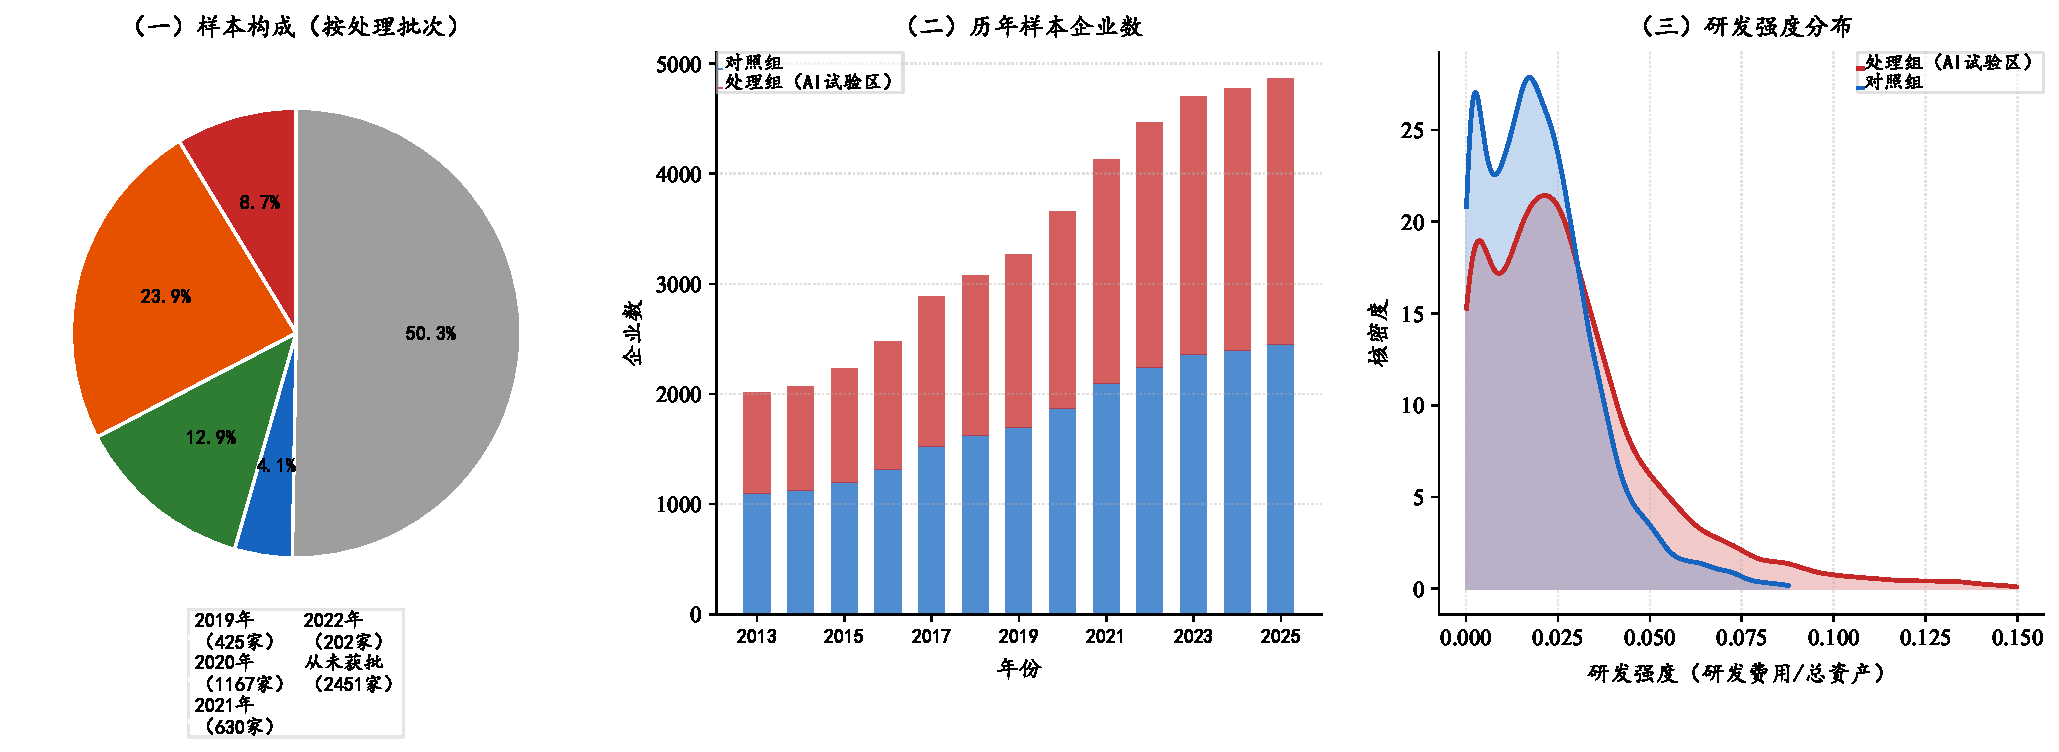
\includegraphics[width=\linewidth]{figures/fig9_样本分布_cn.pdf}
\caption{样本构成与研发强度分布}
\label{fig:sample}
\par\vspace{4pt}
\begin{minipage}{\linewidth}
\zihao{-5}\setlength{\baselineskip}{12pt}
注：左图按企业去重。2020年批次占全部企业的23.9\%，占处理组企业的48.1\%。右图为研发强度分布。
\end{minipage}
\end{figure}

\section{实证策略}

基准式是
\begin{equation}
Y_{it}=\alpha+\beta Treat_{it}+\gamma X_{it}+\mu_i+\lambda_t+\varepsilon_{it}.
\label{eq:main}
\end{equation}
$Y_{it}$是研发强度或资本支出强度。$\mu_i$是企业固定效应，$\lambda_t$是年份固定效应。标准误在企业层面聚类。$\beta$是已获批城市的企业相对于尚未获批或从未获批企业的平均差异。在处理时点交错、处理效应又随批次变化时，这个双向固定效应系数会把“已处理组对后处理组”的比较混进来，权重甚至可以为负\parencite{goodman2021difference,dechaisemartin2020twoway}。

动态式把相对年份做成虚拟变量，窗口与图~\ref{fig:event}一致，取$k=-4,\ldots,4$，去掉$k=-1$：
\begin{equation}
Y_{it}=\alpha+\sum_{k=-4,\,k\neq -1}^{4}\beta_k D_{it}^{k}+\gamma X_{it}+\mu_i+\lambda_t+\varepsilon_{it}.
\label{eq:event}
\end{equation}
前一稿把窗口写成$-6$到$6$。图和作图代码都是$-4$到$4$。

对批次$g\in\{2019,2020,2021,2022\}$，干净比较只保留该批次企业和从未处理企业：
\begin{equation}
Y_{it}=\alpha_g+\delta_g D_{it}^{g}+\gamma_g X_{it}+\mu_i+\lambda_t+\varepsilon_{it}.
\label{eq:cohort}
\end{equation}
$D_{it}^{g}$在企业属于批次$g$且$t\ge g$时为1。这样避免了用已经获批的城市当对照。它仍然是各批次单独的双向固定效应，不是\textcite{callaway2021difference}的组—时间估计量，也没有同时给出四个批次的联合推断。按企业数加权的四个$\delta_g$约为0.00076。这个加权平均没有标准误，后文不把它当作一个可以检验的总效应。

\section{基准结果}

\subsection{平均效应}

表~\ref{tab:main}第（1）列，$Treat$对研发强度的系数为0.0004（$t=1.38$）。相对于研发强度均值0.0254，这是均值的1.6\%，而且不能拒绝零。第（2）列对资本支出强度的系数为$-0.0007$（$t=-0.78$）。H1在全样本上没有得到支持。

\begin{table}[htbp]
\centering
\caption{基准回归}
\label{tab:main}
\begin{threeparttable}
\begin{tabular*}{\textwidth}{@{\extracolsep{\fill}}lcc}
\toprule
 & （1）研发强度 & （2）资本支出强度 \\
\midrule
Treat & 0.0004 & $-$0.0007 \\
 & (0.0003) & (0.0009) \\
 & [1.38] & [$-$0.78] \\
\midrule
控制变量 & 是 & 是 \\
企业固定效应 & 是 & 是 \\
年份固定效应 & 是 & 是 \\
观测数 & 32,910 & 44,474 \\
\bottomrule
\end{tabular*}
\begin{tablenotes}
\item 注：括号内为企业层面聚类标准误，方括号内为$t$值。控制变量为企业规模、杠杆率、资产收益率、企业年龄、现金持有、托宾Q和国有企业虚拟变量。
\end{tablenotes}
\end{threeparttable}
\end{table}

控制变量的方向与常见结果一致：规模、盈利和现金持有的系数为正，杠杆率为负。这些系数不是本文的对象。平均处理效应不显著，不能从控制变量的符号里补回来。

\subsection{动态效应}

图~\ref{fig:event}左图是研发强度。$k=-4$的点估计低于零，随后向基准期$k=-1$回升。各期置信区间较宽，不能说平行趋势已经被拒绝，也不能说图已经把它证实成一条平坦的零线。政策当年和其后两年的点估计为负，第3年和第4年才转到零以上，事后每一期的95\%置信区间仍然覆盖零。前一稿写“第3年起效应接近显著”，图中没有哪一期的置信区间离开零。

右图是资本支出。事后点估计落在零以下，置信区间覆盖零。结论是检测不到系统性变化，不是精确的零效应。

\begin{figure}[htbp]
\centering
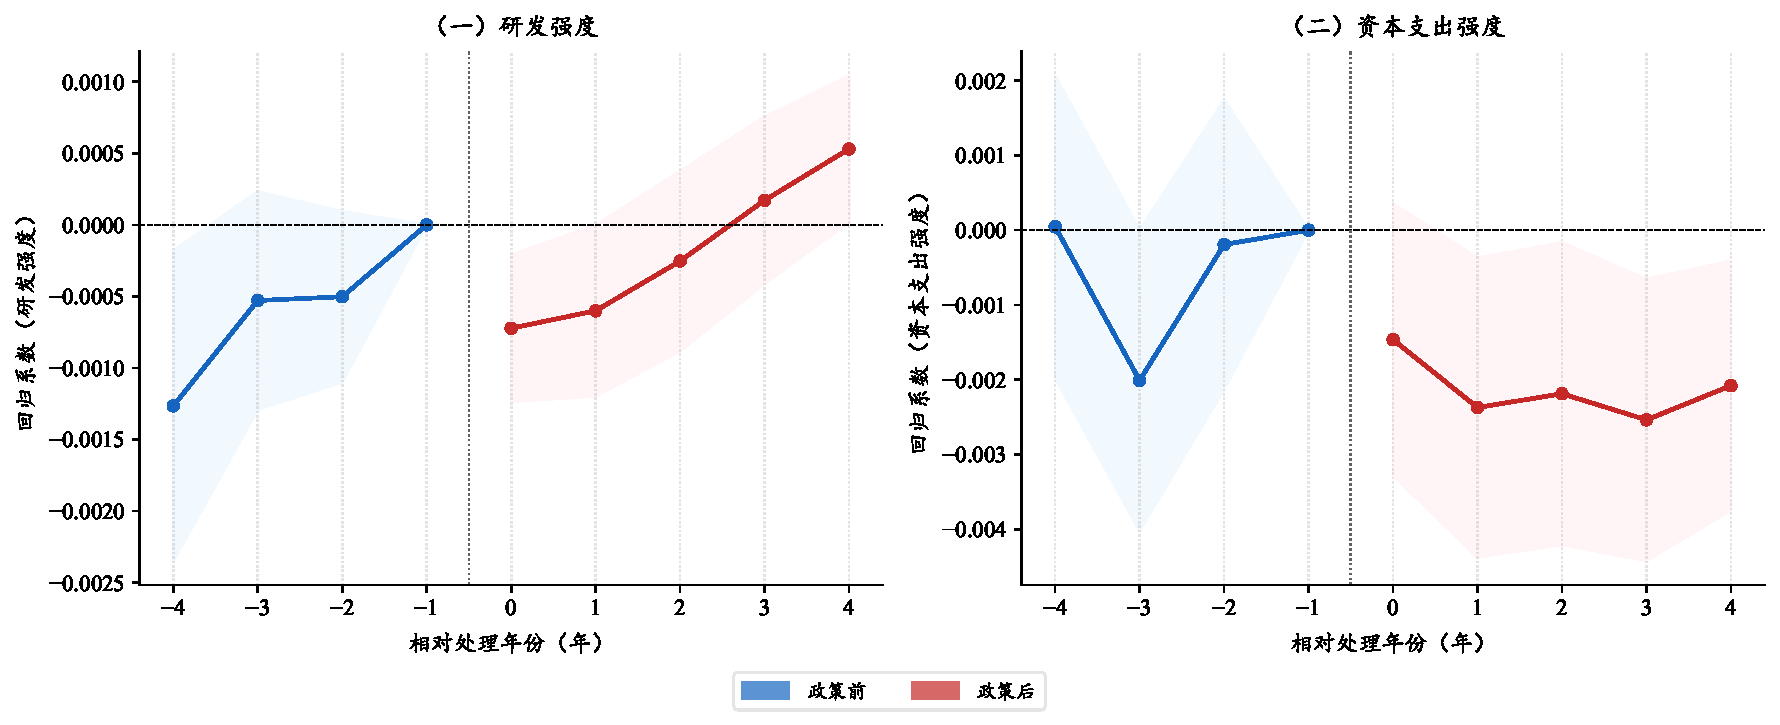
\includegraphics[width=\linewidth]{figures/fig2_事件研究_cn.pdf}
\caption{事件研究}
\label{fig:event}
\par\vspace{4pt}
\begin{minipage}{\linewidth}
\zihao{-5}\setlength{\baselineskip}{12pt}
注：基准期为$t=-1$。窗口为相对年份$-4$至$4$。控制变量和固定效应同表~\ref{tab:main}。阴影为95\%置信区间，标准误在企业层面聚类。
\end{minipage}
\end{figure}

图~\ref{fig:trend}把各批次按获批年对齐后的原始均值叠在一起。它是描述，不是式~\eqref{eq:event}的系数。政策前两组大体同向变动，政策后的分叉不大，和平均效应接近零是一致的。

\begin{figure}[htbp]
\centering
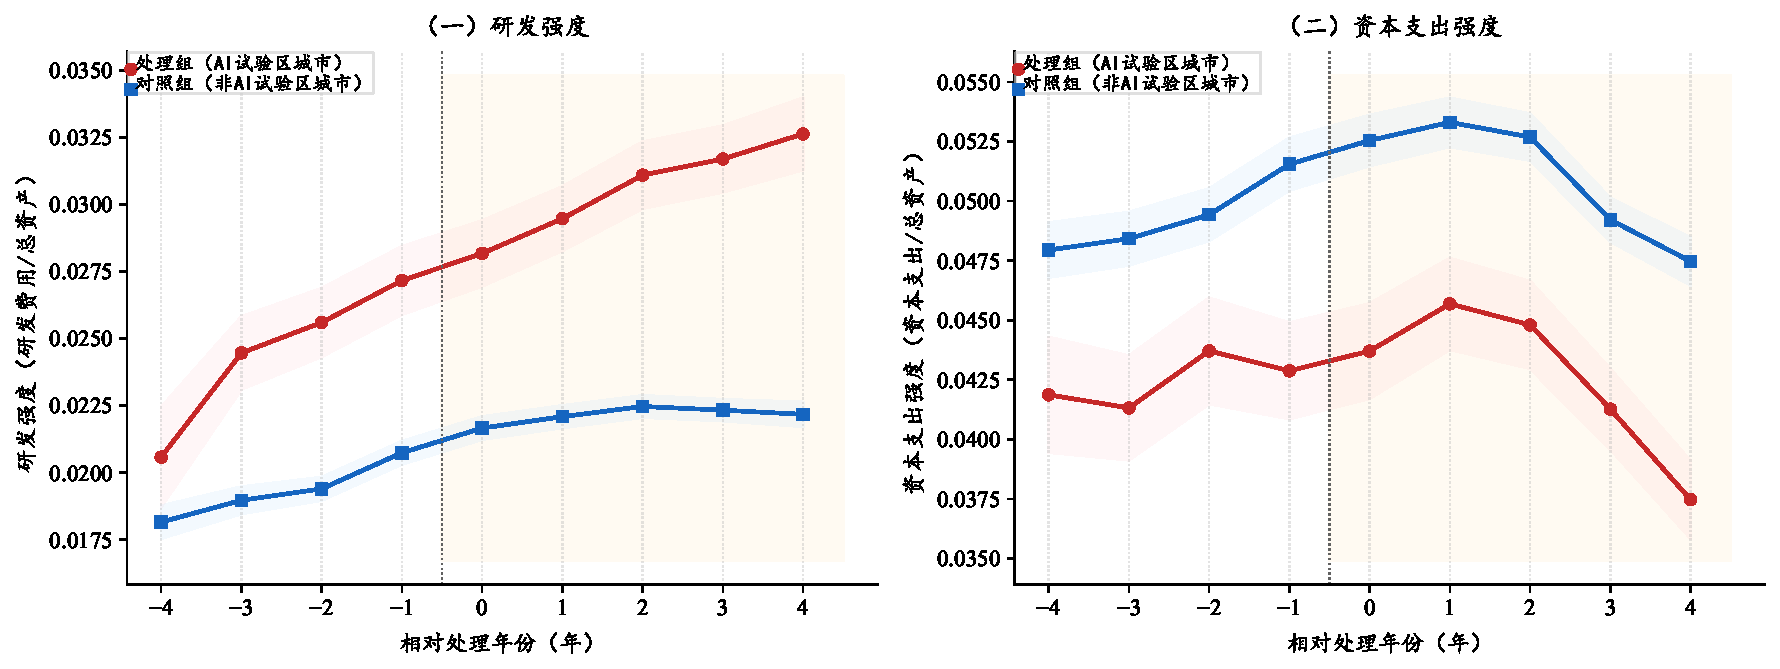
\includegraphics[width=\linewidth]{figures/fig1_趋势图_cn.pdf}
\caption{按获批年份对齐的研发强度与资本支出}
\label{fig:trend}
\par\vspace{4pt}
\begin{minipage}{\linewidth}
\zihao{-5}\setlength{\baselineskip}{12pt}
注：各批次以获批年为$t=0$对齐。对照组为从未获批城市的上市公司。阴影为95\%置信区间。
\end{minipage}
\end{figure}

\section{异质性}

\subsection{批次}

表~\ref{tab:cohort}和图~\ref{fig:cohort}是式~\eqref{eq:cohort}的四个系数。2019年批次0.0023（标准误0.00096，$t=2.38$，企业数399），约合全样本研发强度均值的9\%。2021年批次0.0013（标准误0.00051，$t=2.46$，企业数597），约合均值的5\%。2020年批次0.0001（$t=0.18$，企业数1,108）。2022年批次$-0.0001$（$t=-0.22$，企业数191）。四个$p$值分别为0.017、0.86、0.014和0.83。

企业数小于表~\ref{tab:batch}，是因为这里只用研发回归里出现的公司。2020年进入该回归的1,108家，占这四批企业2,295家的48.3\%。按企业数加权，四个系数的平均是0.00076，没有标准误。

\begin{table}[htbp]
\centering
\caption{分批次与从未处理企业的比较}
\label{tab:cohort}
\begin{threeparttable}
\begin{tabular*}{\textwidth}{@{\extracolsep{\fill}}lcccc}
\toprule
批次 & 企业数 & 系数 & 标准误 & $t$值 \\
\midrule
2019 & 399 & 0.0023 & 0.00096 & 2.38 \\
2020 & 1,108 & 0.0001 & 0.00048 & 0.18 \\
2021 & 597 & 0.0013 & 0.00051 & 2.46 \\
2022 & 191 & $-$0.0001 & 0.00054 & $-$0.22 \\
\midrule
企业数加权 & 2,295 & 0.00076 &  &  \\
\bottomrule
\end{tabular*}
\begin{tablenotes}
\item 注：每个回归只包含该批次企业和从未获批企业，控制变量与固定效应同基准回归。标准误在企业层面聚类。加权平均没有标准误。2019年与2021年的$p$值是0.017和0.014，未做四个批次之间的多重检验校正。
\end{tablenotes}
\end{threeparttable}
\end{table}

\begin{figure}[htbp]
\centering
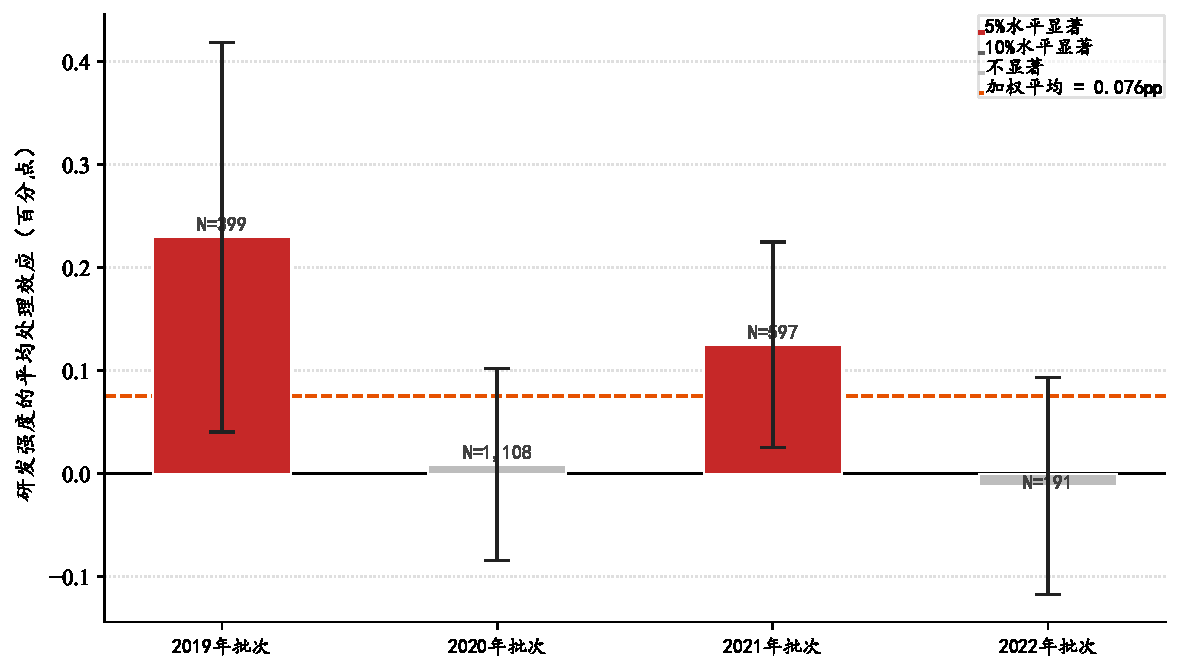
\includegraphics[width=0.85\linewidth]{figures/fig3_cohort_ATT_cn.pdf}
\caption{分批次处理效应}
\label{fig:cohort}
\par\vspace{4pt}
\begin{minipage}{\linewidth}
\zihao{-5}\setlength{\baselineskip}{12pt}
注：纵轴单位是百分点。图中加权平均为0.076个百分点，即0.00076。误差线为95\%置信区间。
\end{minipage}
\end{figure}

这张表说明平均效应接近零，很大程度上是因为最大的2020年批次没有可检测的效应。它没有单独识别出“铺开稀释”。2019年的城市本身就是人工智能活动最密集的一组，2020年的日历时间与疫情重叠，2022年批次到2025年只走完相对年份0到3，而图~\ref{fig:event}里研发点估计要到较后的年份才转到零以上。批次差异是事实，批次差异的原因还没有被分开。

\subsection{行业}

表~\ref{tab:hetero}第（1）列，$Treat\times HighAI$的系数是0.0028（$t=3.74$）。$HighAI$不随时间变化，主效应被企业固定效应吸收，所以$Treat$的主效应$-0.0001$是低暴露行业的政策系数。高暴露子样本中$Treat$为0.0017（$t=2.22$，观测数5,506），低暴露子样本为0.0001（$t=0.27$，观测数27,404）。高暴露行业大约只占研发样本的六分之一，交互项是统计上最强的一个对比。图~\ref{fig:hetero_ind}里，高暴露组在政策前就从大约$-0.004$回升到基准期的零，政策当年的点估计又落到零以下，此后才缓慢转正，各期置信区间仍覆盖零。交互项显著，不能读成政策后出现了一次水平跳跃。它可能混有高暴露行业自己的时间趋势。

\subsection{所有制}

国有企业子样本中$Treat$为$-0.0002$（标准误0.00045，$t=-0.40$，观测数7,738，992家）。民营企业子样本为0.0006（标准误0.00038，$t=1.70$，$p=0.090$，观测数25,171，3,676家）。前一稿正文写民营企业的$t$值为1.50，和系数除以标准误不符；按输出计算是1.70，只在10\%水平边际显著。图~\ref{fig:hetero_soe}相应地把民营企业画得更陡，不能把10\%的子样本系数写成所有制上的确定差异。国有虚拟变量来自实际控制人信息，项目记录里仍把它列为需要核对的变量，所以这一列只作辅助。

\begin{table}[htbp]
\centering
\caption{行业、所有制、杠杆与补贴}
\label{tab:hetero}
\begin{threeparttable}
\begin{tabular*}{\textwidth}{@{\extracolsep{\fill}}lcccc}
\toprule
 & （1）行业 & （2）所有制 & （3）杠杆 & （4）补贴 \\
 & 研发强度 & 研发强度 & 研发强度 & 补贴强度 \\
\midrule
Treat & $-$0.0001 &  & $-$0.0001 & $-$0.0005 \\
 & (0.0004) &  & (0.0004) & (0.00015) \\
 & [$-$0.25] &  &  & [$-$3.43] \\
Treat$\times$HighAI & 0.0028 &  &  &  \\
 & (0.0007) &  &  &  \\
 & [3.74] &  &  &  \\
Treat，国有 &  & $-$0.0002 &  &  \\
 &  & (0.00045) &  &  \\
 &  & [$-$0.40] &  &  \\
Treat，民营 &  & 0.0006 &  &  \\
 &  & (0.00038) &  &  \\
 &  & [1.70] &  &  \\
Treat$\times$高杠杆 &  &  & 0.0009 &  \\
 &  &  & (0.0004) &  \\
 &  &  & [2.10] &  \\
\midrule
控制变量与双向固定效应 & 是 & 是 & 是 & 是 \\
观测数 & 32,910 & 7,738 / 25,171 & 32,910 & 32,909 \\
\bottomrule
\end{tabular*}
\begin{tablenotes}
\item 注：方括号内为$t$值，标准误在企业层面聚类。第（2）列是两个子样本，不是同一个回归里的两项。高杠杆按研发样本杠杆率的中位数划分。补贴回归的系数和$t$值取自项目结果记录。
\end{tablenotes}
\end{threeparttable}
\end{table}

\begin{figure}[htbp]
\centering
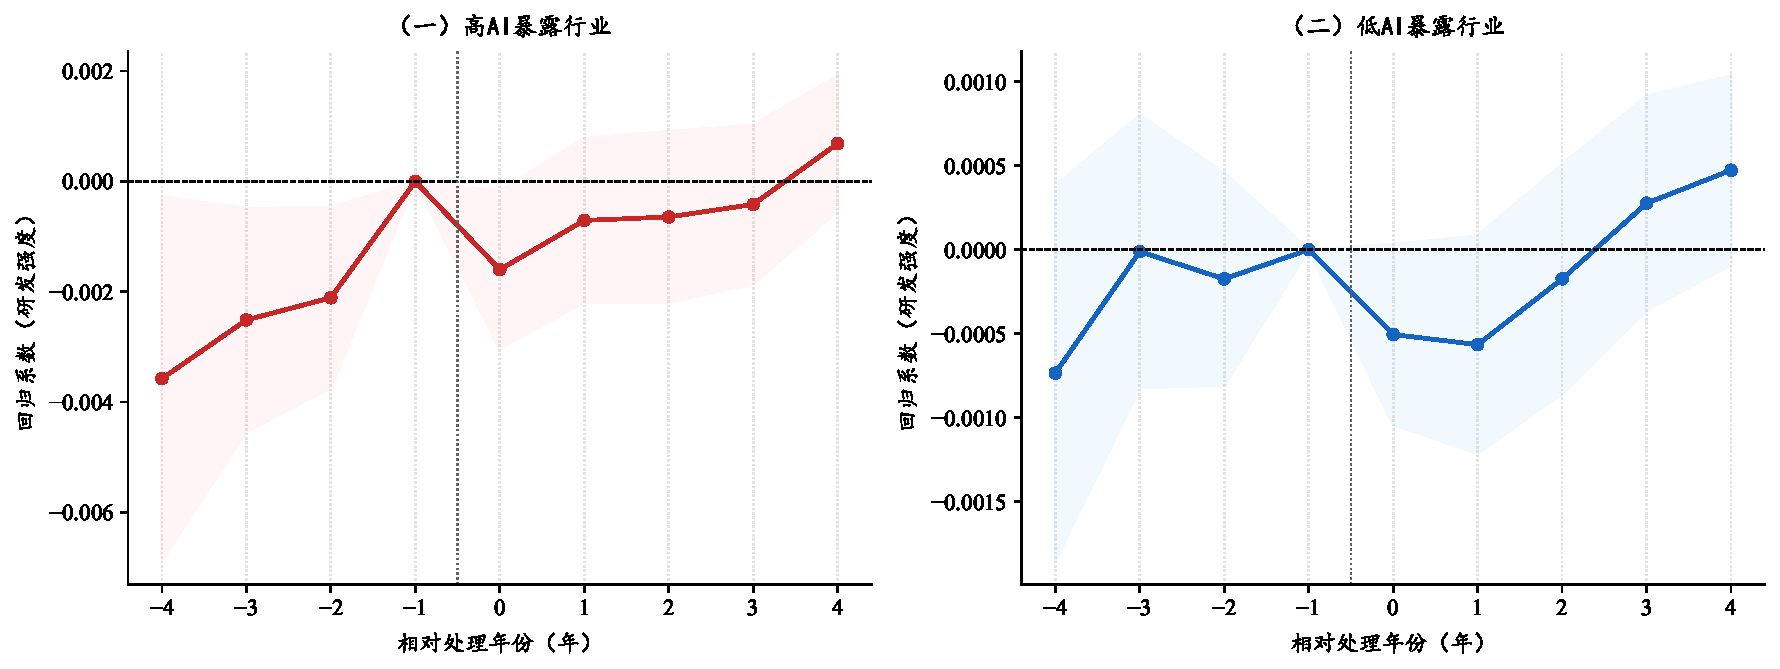
\includegraphics[width=\linewidth]{figures/fig4_异质性_cn.pdf}
\caption{分行业的事件研究}
\label{fig:hetero_ind}
\par\vspace{4pt}
\begin{minipage}{\linewidth}
\zihao{-5}\setlength{\baselineskip}{12pt}
注：高暴露行业为计算机、电子、通信、传媒、医药生物、机械设备、汽车。基准期$t=-1$。阴影为95\%置信区间。
\end{minipage}
\end{figure}

\begin{figure}[htbp]
\centering
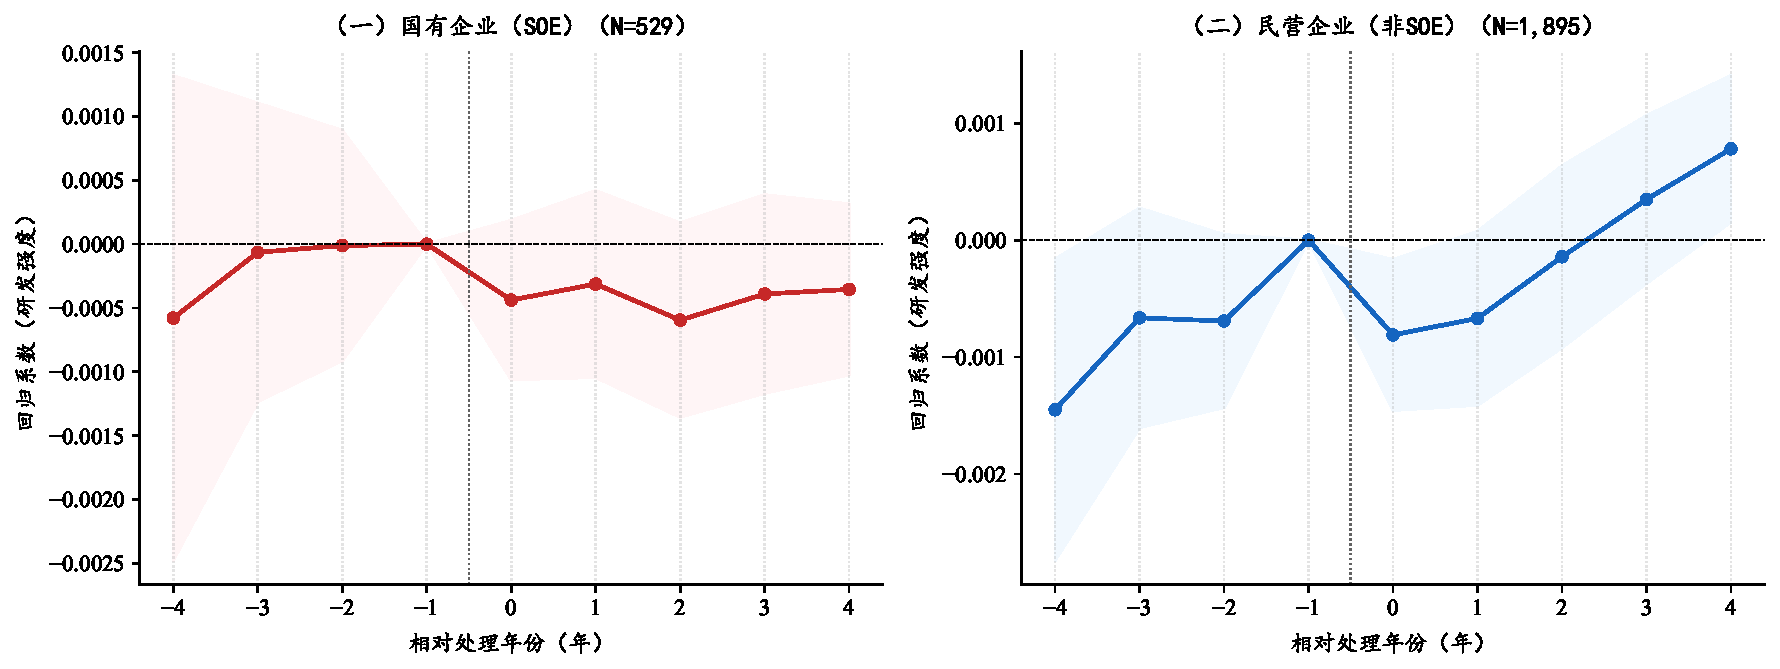
\includegraphics[width=\linewidth]{figures/fig7_所有制_cn.pdf}
\caption{分所有制的事件研究}
\label{fig:hetero_soe}
\par\vspace{4pt}
\begin{minipage}{\linewidth}
\zihao{-5}\setlength{\baselineskip}{12pt}
注：估计式同图~\ref{fig:event}。民营企业子样本的平均系数只在10\%水平边际显著。
\end{minipage}
\end{figure}

\section{机制：补贴与杠杆}

若试验区把钱直接拨给上市公司，补贴强度应当上升。表~\ref{tab:hetero}第（4）列的系数是$-0.0005$（$t=-3.43$）。图~\ref{fig:mechanism}左图里，两组补贴强度在2019年之后没有拉开正向缺口。H2a，就这个代理变量而言，不成立。限制也很具体。变量混有其他收益和营业外收入；钱可以进算力中心、高校和未上市企业，而不会出现在上市公司的营业外项目里；税收优惠也不在这个分子里。负系数拒绝的是“上市公司这笔代理变量上升”，不是“公共支出没有发生”。

杠杆分组与H2b的方向一致。高杠杆子样本的研发系数为0.0011（$t=2.97$），低杠杆子样本为$-0.0005$（$t=-0.99$），交互项0.0009（$t=2.10$）。高杠杆也可能表示企业本来就借得到钱，而不表示它受到约束。本文没有利息率、新增贷款或SA指数。图~\ref{fig:mechanism}右图可以当作分组事实，不能当作信贷渠道已经被估计出来。

\begin{figure}[htbp]
\centering

\includegraphics[width=\linewidth]{figures/fig6_机制_cn.pdf}
\caption{补贴路径与杠杆分组}
\label{fig:mechanism}
\par\vspace{4pt}
\begin{minipage}{\linewidth}
\zihao{-5}\setlength{\baselineskip}{12pt}
注：左图是补贴代理变量的年度均值。右图把高杠杆、低杠杆子样本系数和交互项放在一起。杠杆按样本中位数划分。
\end{minipage}
\end{figure}

\section{稳健性}

表~\ref{tab:robust}的三列替代设定，系数分别是0.0008（$t=1.71$）、0.0006（$t=1.75$）和0.0006（$t=1.67$），都只碰到10\%的临界值。点估计和基准的0.0004同号、同量级，说明平均效应的大小对这几处改动不敏感。显著性对设定敏感，而且没有任何一列达到5\%。这不能用来把基准的“不能拒绝零”改写成“效应稳健为正”。

\begin{table}[htbp]
\centering
\caption{平均效应的替代设定}
\label{tab:robust}
\begin{threeparttable}
\begin{tabular*}{\textwidth}{@{\extracolsep{\fill}}lccc}
\toprule
 & （1）省份$\times$年份 & （2）倾向得分匹配 & （3）去掉直辖市 \\
\midrule
Treat & 0.0008 & 0.0006 & 0.0006 \\
 & [1.71] & [1.75] & [1.67] \\
观测数 & 32,907 & 18,429 & 26,583 \\
\bottomrule
\end{tabular*}
\begin{tablenotes}
\item 注：被解释变量为研发强度。方括号内为$t$值。第（1）列用省份$\times$年份固定效应替换年份固定效应，仍保留企业固定效应。第（2）列在2018年按规模、杠杆、资产收益率和年龄估计倾向得分，最近邻、卡尺0.05，匹配后回归样本为18,429。前一稿写卡尺0.01、样本量11,266，与输出不符。第（3）列去掉北京、上海、天津、重庆。基准系数是0.0004（$t=1.38$）。
\end{tablenotes}
\end{threeparttable}
\end{table}

第（1）列比较的是同一省、同一年里获批城市和未获批城市。系数略大，仍然只在10\%水平。第（3）列去掉四个直辖市后系数没有塌掉。北京、上海、天津属于2019年批次，深圳不是直辖市。这一列只说明平均系数不靠这四个城市的极端值撑着；本文没有在去掉直辖市之后重估四个批次。

图~\ref{fig:placebo}的图例是300次抽取：随机抽出与处理组等量的公司，只保留这些公司原来的$Treat$，其余公司置零。从未处理的公司被抽中后仍然是0，所以这不是把处理时点重新分配的安慰剂。图例写真实系数0.0004高于55.7\%的抽取系数。另一套练习把公司的获批年份打乱，重复500次，真实系数高于55.4\%的伪系数。两套数字都落在分布中部。前一稿写真实系数位于右尾、因而很不可能由噪声产生，和这两套结果相反。平均效应通不过这个检验。

\begin{figure}[htbp]
\centering
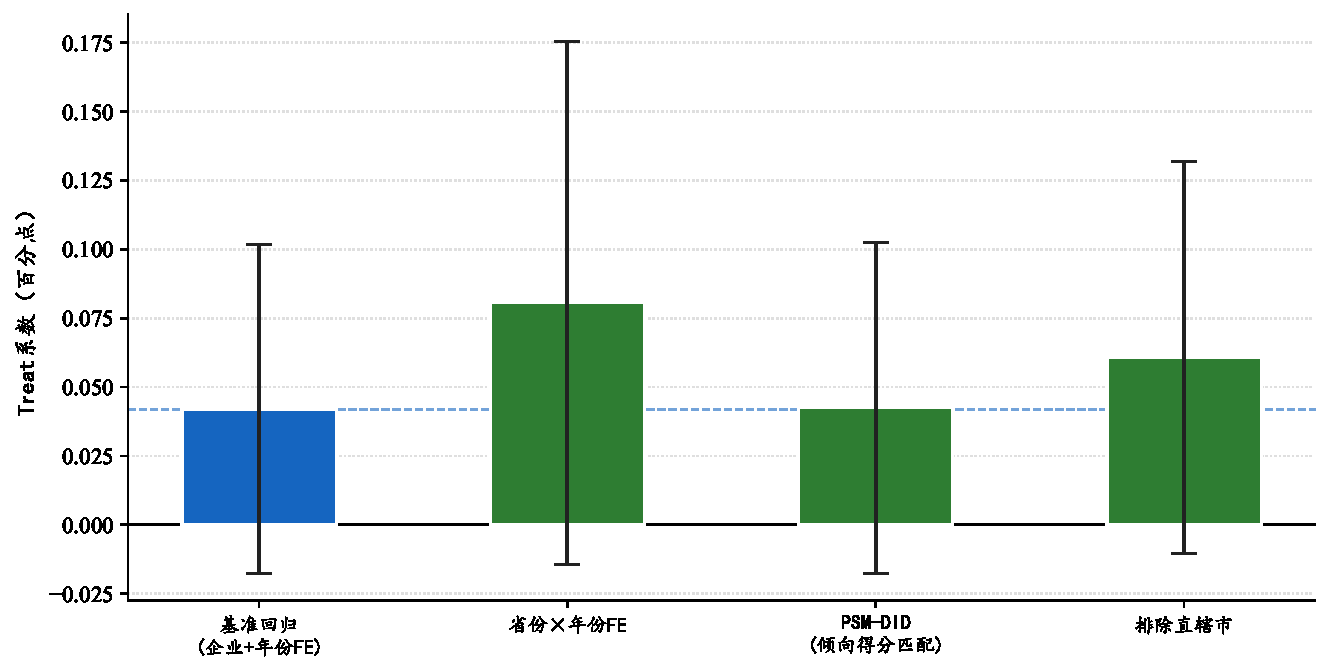
\includegraphics[width=0.82\linewidth]{figures/fig8_稳健性_cn.pdf}
\caption{平均效应在不同设定下的点估计}
\label{fig:robust_coef}
\par\vspace{4pt}
\begin{minipage}{\linewidth}
\zihao{-5}\setlength{\baselineskip}{12pt}
注：被解释变量为研发强度。误差线为95\%置信区间。四条置信区间都覆盖零或贴着零，与“只在10\%水平显著”一致。
\end{minipage}
\end{figure}

\begin{figure}[htbp]
\centering
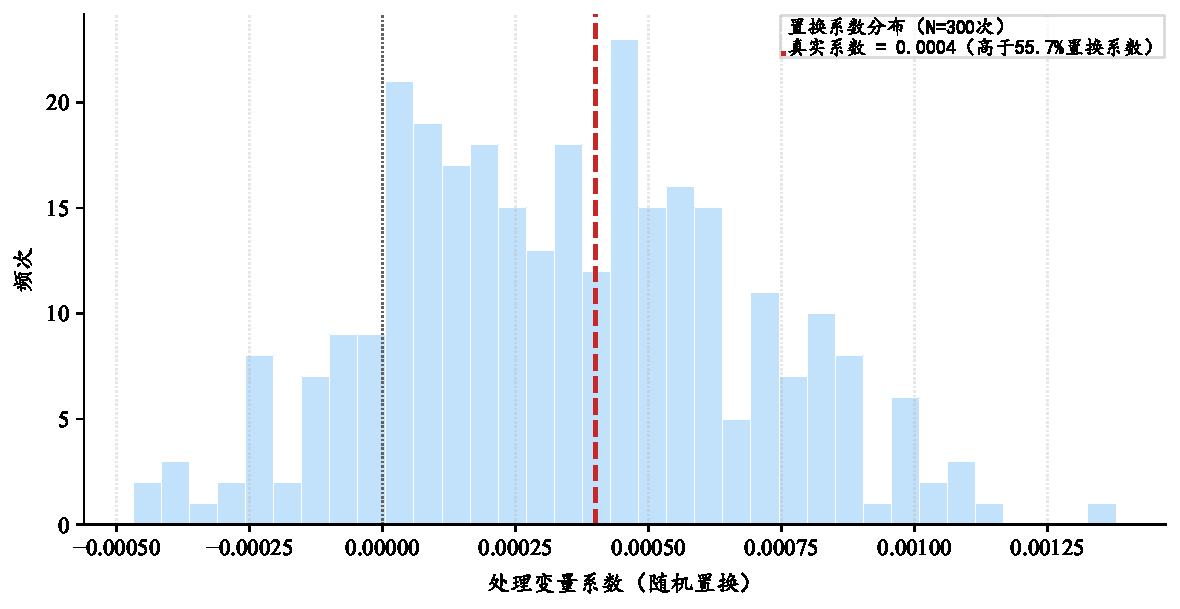
\includegraphics[width=0.78\linewidth]{figures/fig5_安慰剂_cn.pdf}
\caption{图中的300次处理指示抽取}
\label{fig:placebo}
\par\vspace{4pt}
\begin{minipage}{\linewidth}
\zihao{-5}\setlength{\baselineskip}{12pt}
注：该图不是处理时点的完整置换。完整置换见正文：500次打乱获批年份后，真实系数高于55.4\%的伪系数。
\end{minipage}
\end{figure}

\section{结\quad 论}

平均而言，人工智能试验区没有提高上市公司的研发强度，也没有提高资本支出强度。2019年和2021年两个批次的点估计为正，2020年这个最大的批次接近零，所以总体均值被拉低。高人工智能暴露行业有正的交互项。上市公司的补贴代理变量没有上升。高杠杆企业的反应更大，但这不是信贷成本的估计。

这些结果对政策设计的含义应当停在证据停住的地方。第一，不要把全样本的不显著写成政策完全没有作用，也不要把它写成政策总体有效。第二，批次差异值得继续拆，但下一份数据要能把城市原有基础、疫情年份和事后窗口长度分开，而不是把2020年的零效应直接叫作稀释。第三，若公共投入的对象是算力和数据，评估应看到使用这些设施的企业，并单独测量高暴露行业；只看全体上市公司的平均研发，效力太低。第四，要检验融资渠道，需要贷款价格或贷款数量，而不是杠杆率中位数。

本文没有专利和产品数据，注册地也不是研发活动的实际地点，试验区城市不是随机指定的。大约四分之一的观测没有研发记录。四个批次的两个“显著”系数没有经过多重检验校正。平均效应的安慰剂结果位于分布中央。这些限制决定了本文能说的句子：效应依企业和批次而不同，总体均值检测不到，渠道尚未被直接测到。

\printbibliography[title={参考文献}]

\enmaketitle
\end{document}
